



\begin{table}[h]
\begin{tabular}{c|c|l|l|l|}
\cline{2-5}
\textbf{} &
  \multicolumn{2}{p{5cm}|}{\textbf{Only use data collected by current agent}} &
  \multicolumn{2}{c|}{\textbf{Use data collected by other agents}} \\ \hline
\multicolumn{1}{|p{3cm}|}{\textbf{Data collection using current agent}} &

  \multicolumn{2}{l|}{\begin{tabular}[c]{@{}l@{}}
  
Online, on-policy RL \\

  \raisebox{-\totalheight}{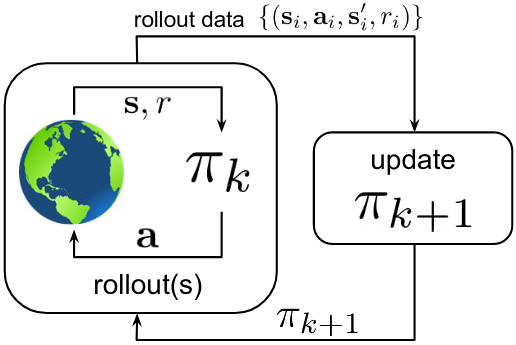
\includegraphics[width=5cm]{figures/on-policy.png}}
  \vspace{5mm} 
  
  \end{tabular}} &
  
  \multicolumn{2}{l|}{\begin{tabular}[c]{@{}l@{}}
  
Online, off-policy RL \\

  \raisebox{-\totalheight}{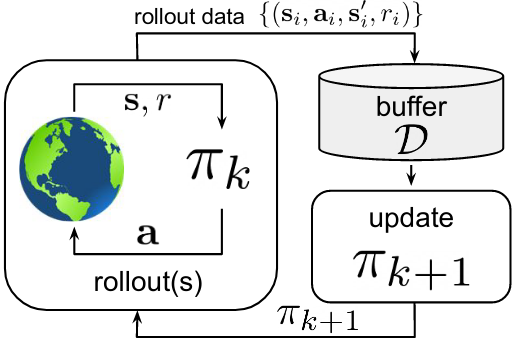
\includegraphics[width=5cm]{figures/off-policy.png}}
  \vspace{5mm} 
  
  \end{tabular}} \\ \hline
  
\multicolumn{1}{|p{3cm}|}{\textbf{Fixed dataset (no additional data collection)}} &
  \multicolumn{2}{c|}
  {-} 
  &
  \multicolumn{2}{l|}{\begin{tabular}[c]{@{}l@{}}
  
  Offline (fully off-policy) RL \\
  
  \raisebox{-\totalheight}{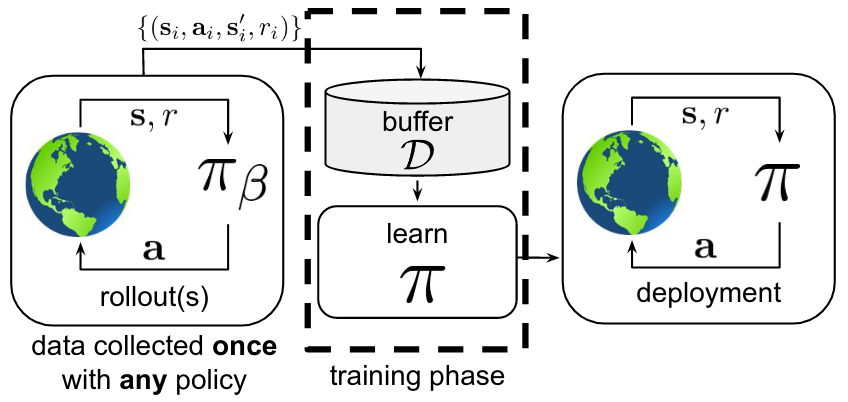
\includegraphics[width=7cm]{figures/offline.png}}
  
  \end{tabular}} \\ \hline
\end{tabular}
\caption{Classification of RL algorithms. Structure of the table from \cite{Google_offline_RL} and figures from \cite{Offline-RL-Levine:2020}.}
\label{tab:RL-classification}
\end{table}





